\chapter{Três Distribuições Fundamentais: Binomial, Gaussiana e Poisson}

\section{A Distribuição Binomial}

Um experimento \textbf{binário} só pode ter dois resultados possíveis, que podem ser interpretados como \textbf{sucesso} ou \textbf{falha}, como por exemplo o lançamento de uma moeda. Mesmo experimentos complexos com um maior número de resultados possíveis podem ser descritos como binários, quando se está simplesmente interessado na ocorrência de um evento específico $A$, ou sua não ocorrência, $A^\complement$. Por exemplo, o lançamento de um dado pode ser interpretado como um experimento binário se estivermos interessados na ocorrência do número seis, ou na ocorrência de qualquer outro número. É de fundamental importância em estatística determinar as propriedades dos experimentos binários, e a distribuição do número de sucessos quando o experimento é repetido várias vezes sob as mesmas condições experimentais. Uma variável aleatória binária é geralmente referida como \textbf{variável de Bernoulli}.

\subsection{Derivação da Distribuição Binomial}

Considere um experimento binário caracterizado por uma probabilidade de sucesso $p$ e, portanto, uma probabilidade de falha $q = 1 - p$. As probabilidades $p$ e $q$ são determinadas de acordo com a teoria da probabilidade e são assumidas como conhecidas para o experimento em questão. Quando o experimento é repetido $N$ vezes nas mesmas condições experimentais, é interessante calcular a probabilidade de obter $n$ sucessos em $N$ tentativas. A ordem em que os $n$ sucessos ocorrem não é relevante; por exemplo, considere lançar uma moeda quatro vezes e estar interessado na probabilidade de exatamente duas dessas jogadas mostrarem cara. O cálculo da probabilidade binomial segue estes passos:
\begin{enumerate}[noitemsep]
\item \textbf{Probabilidade de uma sequência ordenada}. A probabilidade de ter $n$ sucessos e, portanto, $N - n$ falhas ocorrendo em uma ordem específica é dada por:
\begin{equation}\label{3.1}
P(\text{sequência específica de $n$ sucessos}) = p^n \times q^{N-n}.
\end{equation}
Este resultado pode ser visto usando a propriedade de independência entre os $N$ eventos, de modo que as probabilidades individuais podem simplesmente ser multiplicadas.

\item  \textbf{Número de sequências ordenadas ou permutações}. Comece contando quantas sequências ordenadas existem que têm $n$ sucessos em $N$ tentativas. Para começar, cada uma das $N$ tentativas pode resultar no ``primeiro'' sucesso, e portanto existem $N$ possibilidades para qual tentativa será o primeiro sucesso. Continuando para o ``segundo'' sucesso, sobram apenas $N - 1$ possibilidades para qual tentativa será o segundo sucesso, e assim por diante. Este método de contagem de sequências rotula cada sucesso como primeiro, segundo, etc., e leva ao número de permutações de $n$ sucessos em $N$ tentativas:
\begin{equation}\label{3.2}
\text{Perm}(n, N) = N \cdot (N - 1) \cdot (N - n + 1) = \dfrac{N!}{(N - n)!}.
\end{equation}

\begin{exemplo}{}{}
Considere o caso de $n = 2$ sucessos em $N = 4$ tentativas. De acordo com a \autoref{3.2}, o número de permutações é $4!/(4-2)! = 4!/2! = 12$. As 12 sequências ordenadas que resultam em 2 sucessos em 4 tentativas estão listadas na \autoref{tab:3-1}. O símbolo $S_1$ denota o ``primeiro sucesso'' e $S_2$ o ``segundo sucesso''. Considere, por exemplo, as linhas 5 e 8: ambas representam a mesma situação em que as tentativas 2 e 3 resultam em sucesso. Na realidade, elas não são sequências diferentes, mas simplesmente um resultado do método de contagem de sequências ordenadas no tempo.

\begin{center}
	\begin{tabular}{|c|cccc|c|cccc|}
		\hline
		\multirow{2}{*}{Sequência} & \multicolumn{4}{c|}{Número de tentativas}                                        & \multirow{2}{*}{Sequência} & \multicolumn{4}{c|}{Número de tentativas}                                        \\ \cline{2-5} \cline{7-10} 
		& \multicolumn{1}{c|}{1} & \multicolumn{1}{c|}{2} & \multicolumn{1}{c|}{3} & 4     &                            & \multicolumn{1}{c|}{1} & \multicolumn{1}{c|}{2} & \multicolumn{1}{c|}{3} & 4     \\ \hline
		1                          & $S_1$                  & $S_2$                  & --                     & --    & 7                          & $S_2$                  & --                     & $S_1$                  & --    \\ \cline{1-1} \cline{6-6}
		2                          & $S_1$                  & --                     & $S_2$                  & --    & 8                          & --                     & $S_2$                  & $S_1$                  & --    \\ \cline{1-1} \cline{6-6}
		3                          & $S_1$                  & --                     & --                     & $S_2$ & 9                          & --                     & --                     & $S_1$                  & $S_2$ \\ \cline{1-1} \cline{6-6}
		4                          & $S_2$                  & $S_1$                  & --                     & --    & 10                         & $S_2$                  & -                      & --                     & $S_1$ \\ \cline{1-1} \cline{6-6}
		5                          & --                     & $S_1$                  & $S_2$                  & --    & 11                         & --                     & $S_2$                  & --                     & $S_1$ \\ \cline{1-1} \cline{6-6}
		6                          & --                     & $S_1$                  & --                     & $S_2$ & 12                         & --                     & --                     & $S_2$                  & $S_1$ \\ \hline
	\end{tabular}
	\captionof{table}{Ilustração das permutações (sequências ordenadas) de 2 sucessos em 4 tentativas}
	\label{tab:3-1}
\end{center}

\end{exemplo}

\item \textbf{Número de sequências não ordenadas ou combinações}. Como fica claro a partir do exemplo anterior, o número de permutações não é exatamente o número procurado, uma vez que não importa qual sucesso é rotulado como primeiro, segundo, etc. De acordo com a \autoref{3.2}, no caso de $n = N$, há $n!$ maneiras de ordenar $n$ sucessos entre si. Portanto, o número de permutações (ordenadas no tempo) precisa ser dividido por $n!$ para evitar a contagem dupla de sequências equivalentes. Fica claro, portanto, que o número de \textbf{combinações} de $n$ sucessos em $N$ tentativas é:
\begin{equation}\label{3.3}
C(n, N) = \dfrac{\text{Perm}(n, N)}{n!} = \dfrac{N!}{n!(N-n)!} = \binom{N}{n}.
\end{equation}
O número de combinações é o número de sequências possíveis de $n$ sucessos em $N$ tentativas. Esse número, é chamado de \textbf{coeficiente binomial} e é indicado pelo símbolo entre parênteses. O coeficiente binomial é usado na expansão binomial:
\begin{equation}\label{3.4}
(p + q)^N = \sum_{n=0}^{N} \binom{N}{n} p^n q^{N-n}.
\end{equation}

\begin{exemplo}{}{}
Continue a considerar o caso de 2 sucessos em 4 tentativas. Existem $2! = 2$ maneiras de ordenar os 2 sucessos entre si (ou um ou o outro é o primeiro sucesso). Portanto, o número de combinações de 2 sucessos em 4 tentativas é $4!/[2!(4-2)!] = 6$, e não 12. Conforme indicado acima, de fato, cada sequência tinha sua sequência ``gêmea'' listada separadamente, e a \autoref{3.3} conta corretamente apenas sequências diferentes.
\end{exemplo}
\end{enumerate}

De acordo com os resultados obtidos acima, o que resta a ser feito é usar a probabilidade de cada sequência \eqref{3.1} e multiplicá-la pelo número de combinações na \autoref{3.3} para obter a probabilidade geral de ter $n$ sucessos em $N$ tentativas. Isso leva à função massa de probabilidade (FMP):
\begin{equation}\label{3.5}
P_N(n) = \binom{N}{n} p^n q^{N-n}, \quad n = 0, \ldots, N,
\end{equation}
conhecida como a \textbf{distribuição binomial}. Esta distribuição descreve a probabilidade de $n$ sucessos em $N$ tentativas de um experimento binário com probabilidade de sucesso $p$. A \autoref{3.4} mostra que a distribuição binomial é devidamente normalizada. Exemplos da distribuição binomial são mostrados na \autoref{fig:3-1}.

\begin{SCfigure}[\sidecaptionrelwidth][ht!]
	\centering
	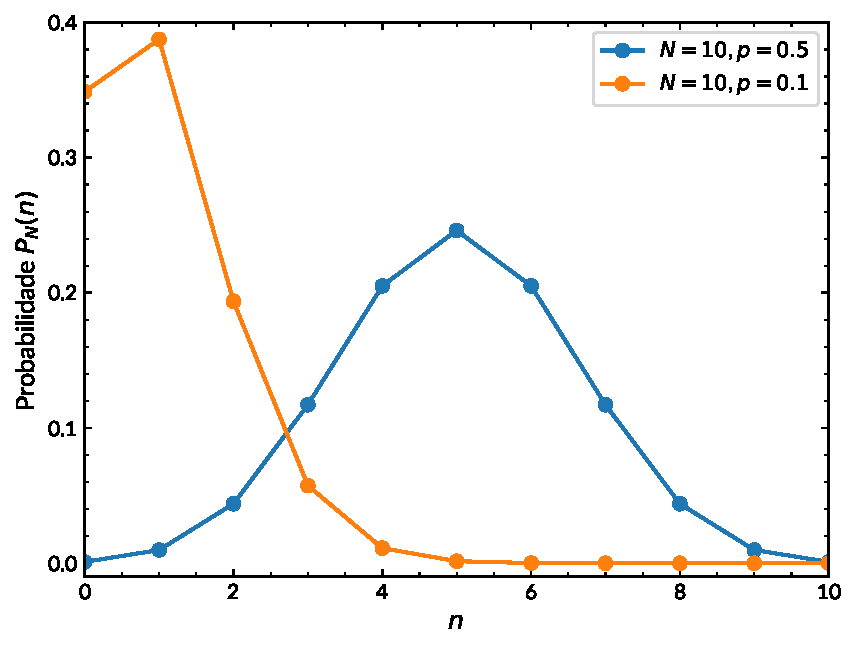
\includegraphics[width=0.7\linewidth]{Figuras/3-1.pdf}
	\caption{Distribuições binomiais de exemplo para $N = 10$ e $p = 0.5$, $p = 0.1$. A função é definida apenas para inteiros não negativos $0 \leq n \leq N$.}
	\label{fig:3-1}
\end{SCfigure}

\subsection{Momentos da Distribuição Binomial}

Os momentos de primeira e segunda ordem de uma variável $X$ distribuída binominalmente são dados por:
\begin{subequations}\label{3.6}
\begin{align}
\mathbb{E}[X] &= \mu = pN \label{3.6a}\\
\mathbb{E}[X^2] &= \mu^2 + pqN 
\end{align}
\end{subequations}
Vamos provar essas equações começando pela média,
\begin{equation*}
\mathbb{E}[X] = \sum_{n=0}^{N} n P_N(n) = \sum_{n=0}^{N} \binom{N}{n} n p^n q^{N-n} = \sum_{n=0}^{N}  \binom{N}{n} \left[p \dfrac{\partial}{\partial p}\right]p^n q^{N-n};
\end{equation*}
O operador linear $p\frac{\partial}{\partial p}$ pode ser aplicado a toda a soma, levando a (considere a substituição da \autoref{3.4} aqui):
\begin{equation*}
\mathbb{E}[X] = p \dfrac{\partial}{\partial p} \sum_{n=0}^{N} \binom{N}{n} p^n q^{N-n} = p \dfrac{\partial}{\partial p} (p + q)^N = pN(p + q)^{N-1} = pN,
\end{equation*}
onde o último passo se deve ao fato de que $p + q = 1$. A derivação para o momento $\mathbb{E}[X^2]$ é similar:
\begin{equation*}
\mathbb{E}[X^2] = \sum_{n=0}^{N} n^2 P_N(n) = \sum_{n=0}^{N} \binom{N}{n} n^2p^n q^{N-n}.
\end{equation*}
Observe que, se $np^n = p\frac{\partial}{\partial p}p^n$, a seguinte expressão é válida:
\begin{equation*}
n^2p^n = p\frac{\partial}{\partial p} \left(np^n\right) = \left(p\frac{\partial}{\partial p}\right)\left(p\frac{\partial}{\partial p}\right)p^n = \left(p\frac{\partial}{\partial p}\right)^2p^n.
\end{equation*}
Assim, 
\begin{align*}
\mathbb{E}[X^2] = \sum_{n=0}^{N} \binom{N}{n} \left(p\frac{\partial}{\partial p}\right)^2 p^nq^{N-n} =  \left(p\frac{\partial}{\partial p}\right)^2 (p + q)^N = p\frac{\partial}{\partial p} \left[pN (p + q)^{N -1}\right].
\end{align*}
Desenvolvendo, 
\begin{align*}
\mathbb{E}[X^2] &= p\left[N(p + q)^{N -1} + pN(N - 1)(p + q)^{N - 2}\right] = pN + (pN)^2 - p^2N \\
&= (pN)^2 + pN(1 - p) = (pN)^2 + pqN,
\end{align*}
onde novamente usamos o fato de que $p + q = 1$. 

Segue-se que a variância da distribuição binomial é dada por:
\begin{equation}\label{3.7}
\sigma^2 = \mathbb{E}[X^2] - \mathbb{E}[X]^2 = (pN)^2 + pqN - (pN)^2 = pqN.
\end{equation}
As equações \eqref{3.6} e \eqref{3.7} descrevem as características mais importantes da distribuição binomial, mostradas na \autoref{fig:3-1} para o caso de $N = 10$. A média é naturalmente dada pelo produto do número de tentativas $N$ e a probabilidade de sucesso \(p\) em cada uma das tentativas.

\begin{exemplo}{}{}
Uma companhia aérea sabe que 5\% das pessoas que fazem reservas não aparecerão no portão de embarque. Para um voo com capacidade para 50 passageiros, a companhia vendeu 52 passagens e quer determinar a probabilidade de que haverá um assento disponível para cada passageiro que aparecer. Utilizando a distribuição binomial, onde cada passageiro tem uma probabilidade $p = 0.95$ de aparecer, queremos calcular a probabilidade de que no máximo 50 dos 52 passageiros compareçam ($P(X \leq 50)$). Definindo $X$ como a variável aleatória que representa o número de passageiros que aparecem, temos $X \sim \text{Binomial}(N = 52, p = 0.95)$. A probabilidade desejada é dada por:
\begin{equation*}
P(X \leq 50) = 1 - P(X = 52) - P(X = 51),
\end{equation*}
onde, usando a fórmula da distribuição binomial \eqref{3.5},
\begin{align*}
P(X = 52) &= \binom{52}{52} (0.95)^{52} (0.05)^0 = (0.95)^{52}\\
P(X = 51) &= \binom{52}{51} (0.95)^{51} (0.05)^1 = 52 \cdot (0.95)^{51} \cdot 0.05.
\end{align*}
Calculando esses valores, obtemos:
\begin{equation*}
P(X \leq 50) = 1 - (0.95)^{52} - 52 \cdot (0.95)^{51} \cdot 0.05 \approx 0.741.
\end{equation*}
Assim, a probabilidade de que haverá um assento disponível para cada passageiro que aparecer é aproximadamente 74.1\%. Consequentemente, a companhia aérea está assumindo um risco de 25.9\% de ter um voo com \textit{overbooking}.
\end{exemplo}

\section{A Distribuição Gaussiana}

A distribuição Gaussiana, frequentemente referida como \textbf{distribuição normal}, desempenha um papel especial na estatística. Uma variável aleatória contínua $X$ é dita ter uma distribuição Gaussiana se sua função densidade de probabilidade (FDP) for
\begin{equation}\label{3.8}
f(x) = \dfrac{1}{\sqrt{2\pi \sigma^2}} \exp\left[-\dfrac{(x-\mu)^2}{2\sigma^2}\right]
\end{equation}
A função de distribuição é definida para todos os valores reais, e sua forma é determinada pelos dois parâmetros $\mu$ e $\sigma^2$, que também representam a média e a variância da variável aleatória (veja a \autoref{fig:3-2}). Uma Gaussiana com parâmetros $\mu$ e $\sigma^2$ é frequentemente referida como $\mathcal{N}(\mu, \sigma^2)$. É útil mostrar que a distribuição Gaussiana pode ser considerada um caso especial da distribuição binomial, no caso de um grande número de experimentos realizados.

\begin{SCfigure}[\sidecaptionrelwidth][ht!]
	\centering
	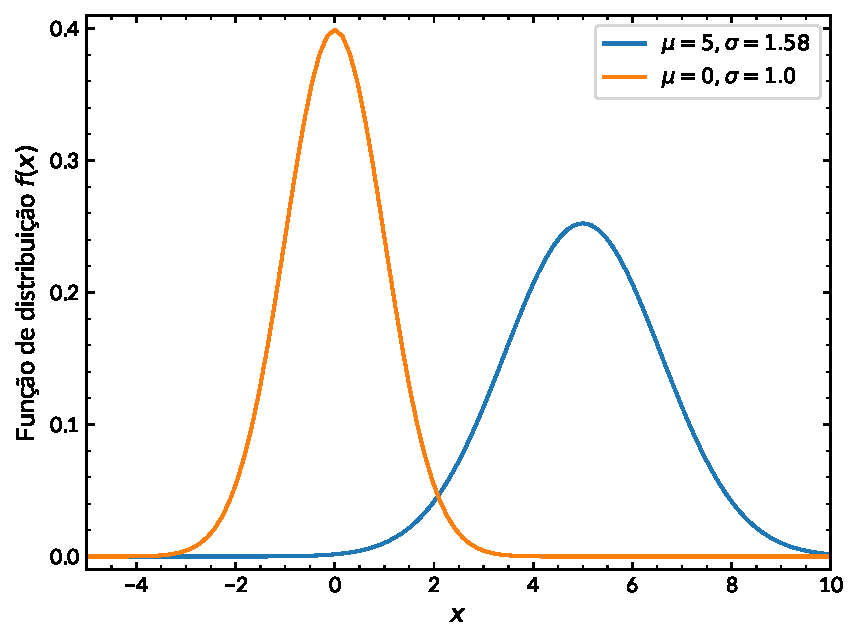
\includegraphics[width=0.7\linewidth]{Figuras/3-2.pdf}
	\caption{Distribuições Gaussianas para valores selecionados da média e variância. A curva Gaussiana em azul tem a mesma média e variância que uma distribuição binomial com $N = 10$ e $p = 0.5$ (mostrada na \autoref{fig:3-1}).}
	\label{fig:3-2}
\end{SCfigure}

\subsection{Derivação da Distribuição Gaussiana a partir da Distribuição Binomial}

Quando o tamanho da amostra $N$ é grande, a distribuição binomial, representada na \autoref{3.5}, assume uma forma mais simplificada. Ter uma expressão analítica alternativa para a distribuição binomial é vantajoso, especialmente considerando a complexidade numérica associada ao cálculo de fatoriais para números grandes. Como destacado na \autoref{fig:3-1}, a distribuição binomial atinge um máximo em torno de $n = Np$. Esta seção demonstra que a distribuição binomial pode ser aproximada por:
\begin{equation}
P_N(n) \approx \dfrac{1}{\sqrt{2\pi Npq}}\exp\left[-\dfrac{(n-Np)^2}{2Npq}\right],
\end{equation}
quando $N \gg 1$, e para valores da variável que estão próximos ao pico da distribuição.

Vamos começar expandindo o logaritmo da probabilidade binomial como uma série de Taylor na vizinhança do valor de pico $\tilde{n}$,
\begin{equation*}
\ln P_N(n) = \ln P_N(\tilde{n}) + \sum_{k=1}^{\infty} \dfrac{B_k}{k!} \Delta n^k,
\end{equation*}
onde $\Delta n = n - \tilde{n}$ é a desvio em relação ao valor de pico e
\begin{equation*}
B_k = \left. \dfrac{\partial^k \ln P_N(n)}{\partial n^k} \right|_{n=\tilde{n}}.
\end{equation*}
Como, por hipótese, $\tilde{n}$ é um ponto de máximo, $B_1 = 0$. Negligenciando termos de ordem superior à segunda, obtém-se a aproximação
\begin{equation*}
\ln P_N(n) \approx \ln P_N(\tilde{n}) + \dfrac{1}{2} B_2 \Delta n^2,
\end{equation*}
onde $B_2$ é negativo, já que $n = \tilde{n}$ é um ponto de máximo. Segue-se que,
\begin{equation*}
P_N(n) \approx P_N(\tilde{n})\exp\left(-\dfrac{|B_2| \Delta n^2}{2}\right).
\end{equation*}
Negligenciar termos de ordem superior em $\Delta n$ significa que a aproximação será particularmente precisa em regiões onde $\Delta n$ é pequeno, ou seja, próximo ao pico da distribuição. Longe do pico, a aproximação não será tão precisa. Para calcular $|B_2|$, façamos
\begin{equation*}
\ln P_N(n) = \ln\left\{\left[\dfrac{N!}{n!(N-n)!}\right] p^n q^{N-n}\right\} =  \ln N! - \ln n! - \ln (N - n)! + n \ln p + (N - n) \ln q,
\end{equation*}
e trate $n$ como uma variável contínua. Esta aproximação é razoável quando $n$ são números grandes, em particular quando a média $Np \gg 1$ e para valores próximos da média. O logaritmo de $n!$ pode ser aproximado pela \textbf{fórmula de Stirling},
\begin{equation*}
\ln n! = n\ln n - n + \mathcal{O}(\ln n),
\end{equation*}
onde $\mathcal{O}$ significa que, para todos os valores suficientemente grandes de $n$, a diferença entre $\ln n!$ e $n\ln n - n$ será no máximo proporcional ao logaritmo. Assim, a derivada dessa expressão pode ser aproximada com segue,
\begin{equation*}
\dfrac{\partial \ln n!}{\partial n} \approx \ln n + n\left(\dfrac{1}{n}\right) - 1 = \ln n.
\end{equation*}
A partir disso, segue-se que a primeira derivada da função de probabilidade, como esperado, é zero no valor de pico,
\begin{equation*}
\left. \dfrac{\partial \ln P_N(n)}{\partial n} \right|_{n=\tilde{n}} = -\ln n + \ln (N - n) + \ln p - \ln q \bigg|_{n=\tilde{n}} = \left. \ln\left[\dfrac{(N - n)p}{nq}\right] \right|_{n=\tilde{n}} = 0
\end{equation*}
de modo que o resultado familiar de,
\begin{equation*}
(N - \tilde{n})p = \tilde{n} q \Rightarrow \tilde{n} (p + q) = Np \Rightarrow  \tilde{n} = Np,
\end{equation*}
é obtido. Isso leva ao cálculo da segunda derivada,
\begin{equation*}
B_2 = \left. \frac{\partial^2 \ln P_N(n)}{\partial n^2} \right|_{n=\tilde{n}} = \dfrac{\partial}{\partial n} \left.\ln\left[\dfrac{(N - n)p}{nq}\right] \right|_{n=\tilde{n}} = \dfrac{\partial}{\partial n} \left[\ln(N - n) - \ln n\right]\bigg|_{n=\tilde{n}} = \left. -\dfrac{1}{N - n} - \dfrac{1}{n} \right|_{n=\tilde{n}},
\end{equation*}
onde,
\begin{equation*}
B_2 = -\dfrac{1}{N - \tilde{n}} - \dfrac{1}{\tilde{n}} = -\dfrac{1}{N(1 - p)} - \dfrac{1}{Np} = -\dfrac{1}{Npq},
\end{equation*}
em que usamos o fato que $p + q = 1$. Finalmente, a constante de normalização $P(\tilde{n})$ pode ser calculada fazendo uso da integral
\begin{equation*}
\int_{-\infty}^{\infty} e^{-ax^2} dx = \sqrt{\dfrac{\pi}{a}}.
\end{equation*}
impondo a condição de normalização da função de distribuição de probabilidade,
\begin{equation*}
P_N(\tilde{n}) \int_{-\infty}^{\infty} \exp{\left(-\dfrac{|B_2| \Delta n^2}{2}\right)}\,d\Delta n = P_N(\tilde{n}) \sqrt{\dfrac{2\pi}{|B_2|}} = 1, 
\end{equation*}
levando a (lembre-se que $|B_2| = 1/(Npq)$),
\begin{equation*}
P_N(\tilde{n}) = \dfrac{1}{\sqrt{2\pi Npq}}.
\end{equation*}
Assim, a aproximação da distribuição binomial para grandes valores de $n$ é, portanto:
\begin{equation*}
P_N(n) \approx \dfrac{1}{\sqrt{2\pi Npq}}\exp\left[-\dfrac{(n - Np)^2}{2Npq}\right].
\end{equation*}

Temos, portanto, que a média de uma distribuição binomial é $\mu = Np$ e a variância é $\sigma^2 = Npq$. Assim, a aproximação da binomial para grandes valores de $n$ pode ser reescrita como se segue,
\begin{equation}
P_N(n) \approx \dfrac{1}{\sqrt{2\pi Npq}}\exp\left[-\dfrac{(n - \mu)^2}{2\sigma^2}\right].
\end{equation}
que é a forma padrão da distribuição Gaussiana quando $n$ é uma variável contínua.

\subsection{Momentos e Propriedades da Distribuição Gaussiana}

Os parâmetros $\mu$ e $\sigma^2$ são, respectivamente, a média e a variância da distribuição Gaussiana. Esses resultados seguem da derivação da distribuição Gaussiana a partir da binomial e podem ser confirmados por cálculo direto das expectâncias a partir da \autoref{3.8}. Também pode ser provado que momentos centrais de ordem ímpar são zero, uma vez que a Gaussiana é simétrica em relação à média. Dado seu amplo uso na estatística, é importante quantificar a ``largura efetiva'' da distribuição Gaussiana em torno de sua média. Para determinar a probabilidade de que uma variável Gaussiana tenha valores em um intervalo de $\pm z\sigma$,
\begin{equation*}
A(z) = \int_{\mu - z \sigma}^{\mu + z \sigma} f(x) \, dx = \dfrac{1}{\sqrt{2\pi\sigma^2}} \int_{\mu - z \sigma}^{\mu + z \sigma}  \exp\left[-\dfrac{(x - \mu)^2}{2\sigma^2}\right] \, dx,
\end{equation*}
podemos começar simplificando essa integral realizando uma mudança de variável. Definimos $t = (x - \mu) / \sigma$, onde $x = \mu + t\sigma$ e $dx = \sigma dt$. Os limites da integral também mudam: quando $x = \mu - z\sigma$, $t = -z$, e quando $x = \mu + z\sigma$, $t = z$. Substituindo na integral, obtemos,
\begin{equation}\label{3.11}
A(z) = \dfrac{1}{\sqrt{2\pi\sigma^2}} \int_{-z}^{z} \exp\left[-\dfrac{(\mu + t\sigma - \mu)^2}{2\sigma^2}\right] \sigma \,dt = \dfrac{1}{\sqrt{2\pi}} \int_{-z}^{z} \exp\left(-\dfrac{t^2}{2}\right) \, dt.
\end{equation}
Veja que probabilidade da variável esteja dentro de $\pm 1\sigma$ da média é $A(1) = 0.683$, ou $68.3\%$. Este intervalo da variável é também referido como um \textbf{intervalo de confiança} com 68,3\% de probabilidade (intervalos de confiança serão estudados em detalhe em capítulos posteriores). A correspondência entre o intervalo $\pm 1\sigma$ e a faixa que abrange 68.3\% da probabilidade aplica-se estritamente apenas à distribuição Gaussiana, para a qual o valor de $\sigma$ é definido pela função de distribuição. No entanto, é prática comum calcular o intervalo de 68.3\% (às vezes arredondado para 68\%) mesmo para aquelas variáveis aleatórias que não seguem estritamente uma distribuição Gaussiana, referindo-se a ele como o intervalo de $1\sigma$. As probabilidades associadas aos intervalos característicos de uma variável Gaussiana são apresentadas na \autoref{tab:3-2}\footnote{Existem tabelas completas de distribuição Gaussiana em diversos livros de estatística e também em muitos sites. Um bom recurso é o site do \textbf{Calculator.net}, que oferece uma calculadora interativa. Você pode acessar a calculadora através do seguinte link: \url{https://www.calculator.net/z-score-calculator.html}. Aqui você pode inserir o valor de $Z$ e obter a probabilidade correspondente.}.

\begin{SCtable}[\sidecaptionrelwidth][!h]
	\centering
	\begin{tabular}{|l|l|}
		\hline
		Intervalo em torno da média & Probabilidade Integrada (\%) \\ \hline
		$\pm 1\sigma$               & 68.27                        \\ \hline
		$\pm 2\sigma$               & 95.45                        \\ \hline
		$\pm 3\sigma$               & 99.73                        \\ \hline
		$\pm 4\sigma$               & 99.99                        \\ \hline
		$\pm 5\sigma$               & $\geq$ 99.9999               \\ \hline
		FWHM (ou $\pm 1.18 \sigma$) & 76.10                        \\ \hline
	\end{tabular}
	\caption{Probabilidade associada a intervalos característicos de uma distribuição gaussiana.}
	\label{tab:3-2}
\end{SCtable}

Todas as distribuições Gaussianas podem ser obtidas a partir da distribuição padrão $\mathcal{N}(0, 1)$ através de uma simples mudança de variável. Se $X$ é uma variável aleatória distribuída como $\mathcal{N}(\mu, \sigma^2)$ e $Z$ uma Gaussiana padrão $N(0, 1)$, então a relação entre $Z$ e $X$ é dada por
\begin{equation}\label{3.12}
Z = \dfrac{X - \mu}{\sigma} \quad \text{(ou } X = \mu + \sigma Z \text{)}.
\end{equation}
A variável $Z$ também é referida como o \textbf{z-score} associado à variável $X$.

A distribuição cumulativa de uma variável normal $\mathcal{N}(0, 1)$ é definida pela seguinte integral:
\begin{equation}\label{3.13}
	 B(z) = \dfrac{1}{\sqrt{2\pi}} \int_{-\infty}^{z} \exp\left(-\frac{t^2}{2}\right)\,dt = \dfrac{1}{2} + \dfrac{A(z)}{2},
\end{equation}
e descreve a probabilidade integrada até o valor $z$, onde $A(z)$, conforme a \autoref{3.11}, representa a probabilidade integrada entre $\pm z$.

A \textbf{meia largura à meia altura}, algumas vezes referida como \textbf{HWHM} (do inglês \textit{half width at half maximum}), é definida como a distância entre o ponto de máximo da função de distribuição de probabilidade (em $x = \mu$) e o ponto onde a distribuição alcança metade do pico. Dessa forma, ao considerar $x = \mu$ na \autoref{3.8}, obtemos
\begin{equation*}
f(\mu) = \dfrac{1}{\sigma\sqrt{2\pi}},
\end{equation*} 
Como queremos encontrar o ponto onde a distribuição alcança metade deste valor máximo, multiplicamos essa expressão por $1/2$ e igualamos esse resultado a \autoref{3.8},
\begin{equation*}
\dfrac{1}{\sigma\sqrt{2\pi}} \exp\left[-\dfrac{(x-\mu)^2}{2\sigma^2}\right] = \dfrac{1}{2\sigma\sqrt{2\pi}}.
\end{equation*}
Após algum algebrismo na expressão acima, encontramos
\begin{equation*}
\text{HWHM} = |x - \mu| = \sigma \sqrt{2 \ln 2} \approx 1.18 \sigma,
\end{equation*}
o que significa que o ponto de meia altura está ligeiramente além de um desvio padrão da média, de ambos os lados da média. Da mesma forma, a \textbf{largura total à meia altura}, ou \textbf{FWHM} (do inglês \textit{full width at half maximum}), é definida como a faixa completa entre os dois pontos de meia altura, e é aproximadamente $2.36 \sigma$.

\section{A Distribuição de Poisson}

A distribuição de Poisson descreve a probabilidade de ocorrência de eventos em experimentos de contagem quando o resultado possível é um número inteiro. A distribuição é, portanto, discreta e pode ser derivada como um caso limite da distribuição binomial.

\subsection{Derivação da Distribuição de Poisson}

A distribuição binomial possui outra aproximação útil quando a probabilidade de sucesso é pequena, $p \ll 1$. Nesse caso, o número de resultados positivos é muito menor do que o número de tentativas, $n \ll N$, e a função fatorial pode ser aproximada como:
\begin{equation*}
N! = N (N - 1) \cdots (N - n + 1) \cdot (N - n)! \approx N^n(N - n)!. 
\end{equation*}
O termo $q^{N - n}$ pode ser aproximado usando:
\begin{equation*}
\ln q^{N - n} = \ln(1 - p)^{N - n} = (N - n) \ln(1 - p) \approx - p(N - n) \approx - pN, 
\end{equation*}
levando a:
\begin{equation*}
q^{N - n} \approx e^{- pN}
\end{equation*}
Essas duas aproximações podem ser usadas na \autoref{3.5} para obter:
\begin{equation}
P_N(n) = \dfrac{N!}{n!(N-n)!} p^n q^{N-n} \approx \dfrac{N^n(N - n)!}{n!(N - n)!}p^n e^{- pN} = \dfrac{(pN)^n}{n!}e^{- pN}.
\end{equation}
Como $pN$ é a média da distribuição, a aproximação torna-se:
\begin{equation}\label{3.15}
P_N(n) = \dfrac{\mu^n}{n!}e^{- \mu}.
\end{equation}
conhecida como \textbf{distribuição de Poisson}. Esta função descreve a probabilidade de obter $n$ resultados positivos, ou contagens, quando o número esperado de resultados é $\mu$. Pode-se ver imediatamente que a distribuição está devidamente normalizada, já que:
\begin{equation*}
\sum_{n=0}^{\infty} \dfrac{\mu^n}{n!} = e^\mu. 
\end{equation*}

Uma característica fundamental desta distribuição é que ela é descrita por apenas um parâmetro, a média $\mu$, em contraste com a distribuição Gaussiana que tinha dois parâmetros. Isso não significa que a distribuição de Poisson não tenha variância -- nesse caso, não seria uma variável aleatória -- mas que a variância pode ser escrita como uma função da média, como será mostrado a seguir.

\subsection{Momentos e Propriedades da Distribuição de Poisson}

A \autoref{3.15} perdeu sua referência ao experimento binomial, restando apenas a média $\mu = Np$ como parâmetro. Usando a definição de média e variância, é fácil provar que uma variável aleatória $X$ que segue uma distribuição de Poisson tem um valor esperado $\mathbb{E}[X] = \mu$ e uma variância $\text{Var}(X) = \mu$. O fato de que a média é igual à variância pode ser visto usando os valores para a binomial, $\mu = Np$ e $\sigma^2 = Npq$; como $p \ll 1$, $q \approx 1$, e $\mu \approx \sigma^2$. Como resultado, a distribuição de Poisson tem apenas um parâmetro que é igual tanto à média quanto à variância.

A média e a variância de uma distribuição de Poisson também podem ser calculadas diretamente a partir da função de massa de probabilidade. A média pode ser calculada da seguinte forma:
\begin{equation*}
	\mathbb{E}[X] = \sum_{n=0}^{N} n P_N(n) = e^{- \mu}\sum_{n=0}^{N} n \dfrac{\mu^n}{n!}  = e^{- \mu} \left(\mu \dfrac{d}{d\mu}\right)\left(\sum_{n=0}^{N}\dfrac{\mu^n}{n!}\right) = \mu.
\end{equation*}
O momento de segunda ordem é:
\begin{equation*}
	\mathbb{E}[X^2] = \sum_{n=0}^{N} n^2 P_N(n) = e^{- \mu}\sum_{n=0}^{N} n^2 \dfrac{\mu^n}{n!} =  e^{- \mu} \left(\mu \dfrac{d}{d\mu}\right)\left(\sum_{n=0}^{N}n\dfrac{\mu^n}{n!}\right) = e^{-\mu} \mu \left[\dfrac{d}{d\mu}(\mu e^{\mu})\right] = \mu + \mu^2.
\end{equation*}
onde a equação para a média foi usada na derivação. Portanto, a variância é:
\begin{equation*}
\text{Var}(X) = \mathbb{E}[X^2] - \mathbb{E}[X]^2 = \mu + \mu^2 - \mu^2 = \mu.
\end{equation*}

A distribuição de Poisson é interpretada como a probabilidade de ocorrência de \(n\) contagens quando a média esperada das contagens é $\mu$. Isso faz da distribuição de Poisson a principal ferramenta estatística para todos os experimentos de \textit{contagem}. Ao contrário da distribuição binomial, que é limitada a valores inteiros $n \leq N$, a distribuição de Poisson é definida para qualquer número inteiro não negativo. A referência ao número total de eventos possíveis ($N$) e a probabilidade de ocorrência de cada evento ($p$) foi perdida, restando apenas a média $\mu$ para descrever a principal propriedade do experimento de contagem.

Como pode ser visto na \autoref{fig:3-3}, a distribuição de Poisson não é simétrica em relação à média, e a distribuição torna-se mais simétrica para valores maiores da média. Como em todas as distribuições discretas, só é significativo calcular a probabilidade em um ponto específico ou para um conjunto de pontos, e não para um intervalo de pontos, como no caso das distribuições contínuas. Além disso, a média da própria distribuição pode ser um número não inteiro, e ainda assim o resultado do experimento descrito pela distribuição de Poisson só pode assumir valores inteiros.

\begin{SCfigure}[\sidecaptionrelwidth][ht!]
	\centering
	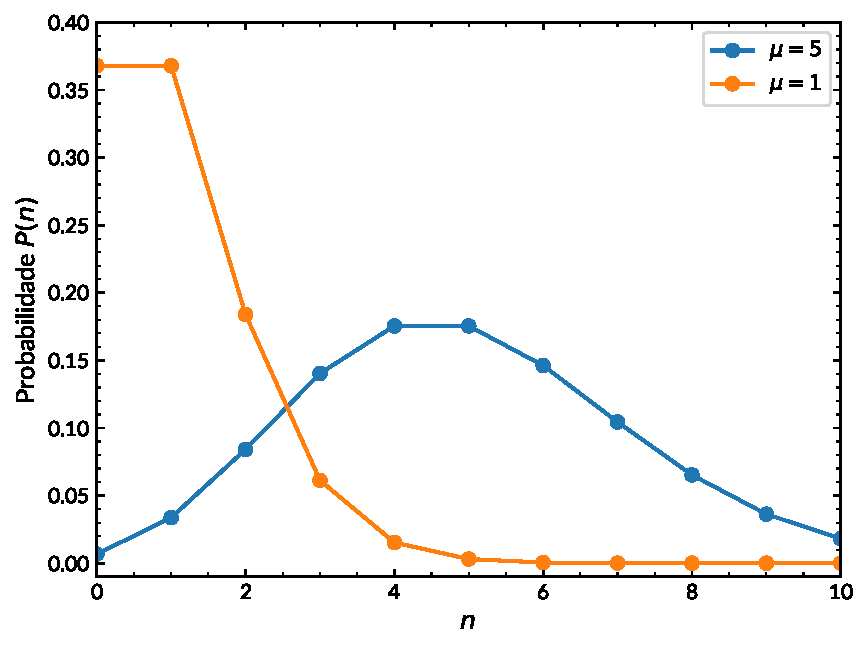
\includegraphics[width=0.7\linewidth]{Figuras/3-3.pdf}
	\caption{Distribuições de Poisson amostrais para valores selecionados da média. A função de massa de probabilidade de Poisson é definida para todos os valores $n \geq 0$.}
	\label{fig:3-3}
\end{SCfigure}

\begin{exemplo}{}{}
Considere uma fonte astronômica conhecida por produzir fótons, que são geralmente detectados por um dado detector na quantidade de $\mu = 2.5$ em um dado intervalo de tempo. A probabilidade de detectar $n = 4$ fótons em um dado intervalo de tempo é, portanto:
\begin{equation*}
P(n = 4; \mu = 2.5) =  \dfrac{\mu^n}{n!}e^{- \mu} = \frac{2.5^4}{4!}e^{-2.5} = 0.134.
\end{equation*}
A razão para uma probabilidade aparentemente grande de obter uma medida que difere da média esperada é simplesmente devido à natureza estatística do processo de detecção.
\end{exemplo}

\subsection{A Distribuição de Poisson e o Processo de Poisson}

Uma justificativa mais formal para a interpretação da distribuição de Poisson como a distribuição de experimentos de contagem vem do \textbf{processo de Poisson}. Embora um tratamento completo deste assunto esteja além do escopo deste livro, uma breve descrição de processos estocásticos servirá para fortalecer a interpretação de \ref{3.15}, que é um dos fundamentos da estatística. Mais detalhes sobre processos estocásticos podem ser encontrados, por exemplo, no livro-texto de \citet{ross2019introduction}.


Um \textbf{processo de contagem estocástico} $\{N(t), t > 0\}$ é uma sequência de variáveis aleatórias $N(t)$, em que $t$ indica o tempo, e $N(t)$ é uma variável aleatória que indica o número de eventos que ocorreram até o tempo $t$. O processo estocástico pode ser pensado como a repetição do experimento de ``contar a ocorrência de um determinado evento'' em vários momentos $t$ e $N(t)$ é o resultado do experimento. O \textbf{processo de Poisson com taxa} $\lambda$ é um tipo particular de processo estocástico, com as seguintes propriedades:

\begin{enumerate}[noitemsep]
\item  $N(0) = 0$, o que significa que no tempo $0$ não há contagens detectadas.
\item O processo tem \textbf{incrementos independentes}, o que significa que $N(s + t) - N(s)$ é independente de $N(s)$. Esta propriedade significa que eventos que ocorrem após o tempo $s$ não são influenciados pelos que ocorreram antes.
\item O processo tem \textbf{incrementos estacionários}, ou seja, a distribuição do número de eventos em um intervalo de tempo $s$ depende apenas da duração do próprio intervalo de tempo.
\item $P(N(h) = 1) = \lambda h + \mathcal{O}(h)$, onde $\mathcal{O}(h)$ é uma função com a propriedade que
\begin{equation*}
\lim_{h \to 0} \dfrac{O(h)}{h} = 0.
\end{equation*}
\item $P(N(h) \geq 2) = \mathcal{O}(h)$. As duas últimas propriedades significam que a probabilidade de obter uma contagem depende do valor finito $\lambda$, enquanto é improvável que dois ou mais eventos ocorram em um curto intervalo de tempo.
\end{enumerate}
Pode-se mostrar que, sob essas hipóteses, o número de eventos $N(t)$ registrado em qualquer intervalo de comprimento $t$ é distribuído segundo Poisson,
\begin{equation}
P\{N(s + t) - N(s) = n\} = \dfrac{(\lambda t)^n }{n!}e^{-\lambda t}
\end{equation}
Isso mostra que a distribuição de Poisson deve ser interpretada como a distribuição da ocorrência de $n$ eventos durante um intervalo de tempo $t$, sob a hipótese de que a taxa de ocorrência de eventos é $\lambda$. Esta interpretação é idêntica à fornecida acima, dado que $\mu = \lambda t$ é a média das contagens nesse intervalo de tempo.

\section{Comparação das Distribuições Binomial, Gaussiana e de Poisson}

Uma comparação entre as distribuições binomial, gaussiana e de Poisson com a mesma média é ilustrada na \autoref{fig:3-4}.

\begin{SCfigure}[\sidecaptionrelwidth][ht!]
	\centering
	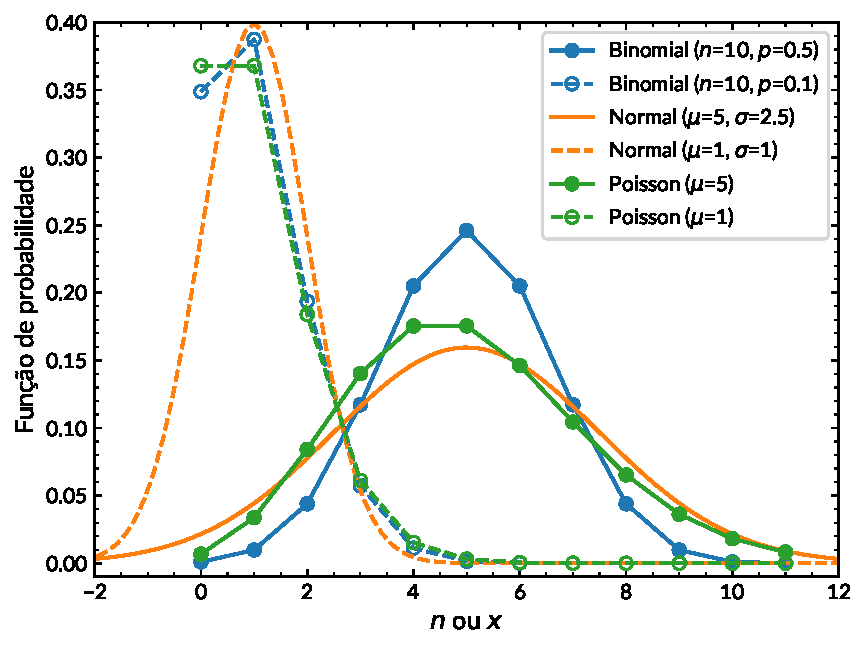
\includegraphics[width=0.7\linewidth]{Figuras/3-4.pdf}
	\caption{Comparação das distribuições de probabilidade binomial, gaussiana e de Poisson. As curvas à esquerda são para variáveis aleatórias com uma média esperada de $\mu = 1$ e à direita para $\mu = 5$.}
	\label{fig:3-4}
\end{SCfigure}

A média e a variância de uma distribuição binomial são determinadas pela escolha do número de tentativas $N$ e pela probabilidade de sucesso $p$ do experimento binário, com $\mu = Np$ e $\sigma^2 = Npq$. No caso da distribuição gaussiana, a média e a variância podem ser escolhidas independentemente como os dois parâmetros da função de distribuição de probabilidade. A distribuição de Poisson, por outro lado, tem a característica especial de ter o mesmo valor para a média e a variância, na quantidade do único parâmetro $\mu$ na distribuição. Os dois conjuntos de curvas na \autoref{fig:3-4} compartilham a mesma média, mas não é possível impor simultaneamente a mesma variância. Por exemplo, a distribuição de Poisson com $\mu = 5$ tem uma variância maior do que a binomial com $N = 10$ e $p = 0.5$, que tem uma variância de $\sigma^2 = 2.5$.

\section{Problemas}

\begin{enumerate}[label=\textbf{\arabic{chapter}.\arabic*.}]
	
\item Considere uma variável aleatória $X$ que segue a distribuição gaussiana:
\begin{equation*}
f(x) = \dfrac{1}{\sqrt{2\pi \sigma^2}} \exp\left[-\dfrac{(x-\mu)^2}{2\sigma^2}\right]
\end{equation*}
Calcule a média e a variância de $X$ e mostre que todos os momentos ímpares $\mathbb{E}[(X - \mu)^n]$ de ordem $n \geq 3$ são zero.

\item Assuma que os resultados de um teste de Q.I. seguem uma distribuição gaussiana, e que as pontuações são padronizadas de tal forma que a média é $\mu = 100$ e o desvio padrão é $\sigma = 15$. Calcule (a) a probabilidade de que uma pontuação de Q.I. seja maior ou igual a 145 e (b) a probabilidade de que a média da pontuação de Q.I. de uma amostra de 100 pessoas, escolhidas aleatoriamente, seja igual ou maior que 105.

\item Uma moeda é lançada dez vezes. Encontre (a) a probabilidade de obter 5 caras e 5 coroas,
(b) a probabilidade de que as primeiras 5 jogadas mostrem caras, e as últimas 5 jogadas mostrem coroas e (c) a probabilidade de obter pelo menos 7 caras.

\item Em um determinado curso, sabe-se que 7.3\% dos alunos reprovam. (a) Qual é o valor esperado de reprovações em uma turma de 32 alunos? (b) Qual é a probabilidade de que 5 ou mais alunos reprovem?

\item A frequência de gêmeos na população europeia é de cerca de 12 em cada 1000 maternidades. Calcule a probabilidade de não haver gêmeos em 200 nascimentos, usando (a) a distribuição binomial e (b) a distribuição de Poisson.
\end{enumerate}